\documentclass{report}
\usepackage[margin=1.3 in]{geometry}
\usepackage{graphicx}
\usepackage{amsmath}
\usepackage[most]{tcolorbox}
\begin{document}
\tableofcontents
\chapter{ Cryptography }
\section{ What is cryptography}

%-------defination----------
\Large{ Cryptography is the science of secret communications.
It is the study of secure communications techniques that allow only the sender and intended recipient of a message to view its contents. The term is derived from the Greek word kryptos, which means hidden. It is closely associated to encryption, which is the act of scrambling ordinary text into what's known as ciphertext and then back again upon arrival. In addition, cryptography also covers the obfuscation of information in images using techniques such as microdots or merging. Ancient Egyptians were known to use these methods in complex hieroglyphics, and Roman Emperor Julius Caesar is credited with using one of the first modern ciphers.


Long before the information age, cryptography was used only to ensure secrecy of information. Encryption was used to ensure confidentiality in communications by spies, military leaders and diplomats. The Egyptian hieroglyphs, the scytale transposition cipher used by the Spartans of Greece, waxed seals and different physical devices to assist with ciphers were used throughout history right up to modern times. These devices underwent further changes when computers and electronics came into the picture, immensely helping in cryptanalysis.Cryptography has become more mathematical now and also finds applications in day-to-day security. It helps you safely transfer or withdraw money electronically and you’d be hard-pressed to come across an individual without a credit or debit card. The public-key encryption system introduced the concept of digital signatures and electronic credentials. Cryptography has a definitive existence in our lives today and the whole system will crumble in its absence. Let’s now discuss the varied uses of cryptography in modern times and its intersection with computer science.
\begin{center}
\includegraphics[scale=0.4]{"crypto.png"}
\end{center}

%---------usage------------------
\section{Usage of cryptography}
\subsection{Secrecy in transmission}
\Large{The major goal of cryptography is to prevent data from being read by any third party. Most transmission systems use a private-key cryptosystem. This system uses a secret key to encrypt and decrypt data which is shared between the sender and receiver. The private keys are distributed and destroyed periodically. One must secure the key from unauthorized access, because any party that has the key can decrypt the encrypted information.}\\

\begin{center}
\includegraphics[scale=0.6]{"public_private.png"}
\end{center}

\Large{Alternately a key-generating-key, called a master key, can be used to electronically generate a one-time session-key for every transaction. The secrecy of the master-key should be maintained by all parties privy to the information. The disadvantage of this method is there’s too much hope riding on the master-key, which if cracked, collapses the entire system.

 

A better method is to use a public-key cryptosystem. In this system, data can be encrypted by anyone with the public-key, but it can be decrypted only by using the private-key, and data that is signed with the private key can be verified only with the public key. With the development of publickey systems, secrecy can be maintained without having to keep track of a large number of keys or sharing a common master-key. If, say, Alex wants to communicate with Neil, she first generates her public/private key pair and sends the public key to Neil over a non-secure channel. Neil  to encrypt information and sends it back to Alex. Only Alex has the private key with which she can decrypt the information. Anyone who intercepts the public key or the encrypted data can’t decrypt the message due to the protocols followed during information transfer.}


\subsection{Secrecy in storage}

\Large{Storage encryption refers to the application of cryptographic techniques on data, both during transit and while on storage media. Storage encryption is gaining popularity among enterprises that use storage area networks (SANs). Secrecy in storage is maintained by storing data in encrypted form. The user has to provide the key to the computer only at the beginning of a session to access the data and it then takes care of encryption and decryption throughout the course of normal use. Hardware devices can also be used for PCs to automatically encrypt all information stored on disk. When the computer is turned on, the user must supply a key to the encryption hardware. The information is plain gibberish without its key thus preventing misuse if the disk is stolen.}

\begin{center}
\includegraphics[scale=0.6]{"file_encryption.png"}
\end{center}

\Large{Multiple ciphers can be used for individual files and folders. The ciphers and keys should be changed frequently to ensure security of data. However, if the user forgets a key, all of the information encrypted with it makes no sense and is rendered useless. This is why backups of encrypted information are advised to be stored in plaintext. The data is only encrypted while in storage, not when in use. This leaves a loophole for the attackers. The system is vulnerable to a security breach if the encryption and decryption are done in software, or if the key is stored somewhere in the system.



\subsection{Integrity in transmission}
\Large{We can use cryptography to provide a means to ensure that data is not altered during transmission, i.e. its integrity is preserved. In electronic funds transfer, it is very important that integrity be maintained. A bank can lose millions if a transaction is illicitly intercepted. Cryptographic techniques are employed to prevent accidental or intentional modification of data during transmission, leading to erroneous actions. One of the ways to ensure integrity is to perform a checksum on the information being transmitted and to transmit the checksum in an encrypted form as well.

The information is received on the other end and again checksummed. The transmitted checksum is decrypted and compared with the previous checksum. If the checksums agree, the information is most likely unaltered. The problem with this scheme is that the checksum of the original message can be known and another message with the same checksum can be generated and sent instead of the original one. This problem can be overcome by using a public-key cryptosystem. After generating the public-key/private-key pair, if we throw away the private-key and use only the public-key to encrypt the checksum, the checksum becomes impossible to decrypt. In order to verify the checksum, we generate a new checksum for the received information, encrypt it using the public-key and match it with the encrypted checksum. This is also known as a one-way function as it is hard to invert.}

\subsection{Integrity in storage}

\Large{Integrity in storage had been ensured by access control systems with lock and keys and other guards to prevent unauthorized access to stored data. The existence of computer viruses has changed the scenario and the need of integrity against intentional attack has become a problem of epic proportions. Cryptographic checksums to ascertain validity of stored data are of help here. As in the case of transmission, a cryptographic checksum is produced and compared to the expected value. However, storage media are more vulnerable to attacks than transmission channels due to longer exposure and larger volumes of information.}


\subsection{Authentication of identity}
\Large{Authentication is the process of verifying if the user has enough authority for data access. Simple passwords are used to identify someone. You must also have seen in classic gangster movies, the exchange of keywords to prove identity. Cryptography is similar to the practice of providing passwords for identity authentication. Modern systems use cryptographic transforms in conjunction with other characteristics of individuals to provide more reliable and efficient authentication of identity. Many systems allow passwords to be stored in an encrypted form, with read access available to all programs which may use them. Since passwords are not stored as plaintext, an accidental of data doesn’t compromise the system’s security.Passwords are analogous to the key in a cryptosystem that allows encryption and decryption of anything the password has access to. The principal element of this system is the password selection process. And that’s a whole other subject that we can’t cover here. But in a nutshell, the longer the password, the more random it will be and the harder it is to guess. So if you think it’s easy for you to remember, you should know that it will be all the easier to crack.}

\subsection{Digital signatures}

\Large{A digital signature is a mechanism by which a message is authenticated i.e. proving that a message is coming from a given sender, much like a signature on a paper document. To be as effective as a signature on paper, digital signatures must be hard to forge and accepted in a court of law as binding upon all parties to the transaction. The need for digital signatures arises when the parties dealing in a transaction are not physically close, and the volume of paperwork is high, in other words big business dealings. Digital signatures can be created using a public key cryptosystem and hashing process. }\\
\begin{center}
\includegraphics[scale=0.6]{"digital_sig.png"}
\end{center}

\Large{Hashing produces a message digest that is a small and unique representation of the original message. Hashing is a one-way algorithm, i.e. the message can’t be derived from the digest. Let’s say that Alex is sending a message to Neil. Alex first hashes the message to produce a digest, and then encrypts the digest with her private-key to create her personal signature; the public-key and hash algorithm are appended to it. The whole message including the digest is then encrypted using a one-time symmetric-key which is known only to Alex and Neil. Neil decrypts the message using the symmetric-key. He then decrypts the message digest using the public-key. He would then hash the original message using the same hash algorithm (whose name was appended in the message) with which it was previously hashed. If the evaluated digest and decrypted digest match, then the signature has been verified and the recipient would be sure that the message integrity has been preserved.

Another aspect of this system is the non-repudiation of digital signatures. Since the private-key is only privy to the sender, he can’t deny signing the message. Also, a digital signature can be verified by anyone using the sender’s public-key which is usually included in the digital signature format.}
%----type----
\section{Types of cryptography}
In general there are three types Of cryptography:
\subsection{Symmetric Key Cryptography:}
\Large{It is an encryption system where the sender and receiver of message use a single common key to encrypt and decrypt messages. Symmetric Key Systems are faster and simpler but the problem is that sender and receiver have to somehow exchange key in a secure manner. The most popular symmetric key cryptography system is Data Encryption System(DES).}
\subsection{Hash Functions:}
\Large{There is no usage of any key in this algorithm. A hash value with fixed length is calculated as per the plain text which makes it impossible for contents of plain text to be recovered. Many operating systems use hash functions to encrypt passwords.}

\subsection{Asymmetric Key Cryptography:}
\Large{Under this system a pair of keys is used to encrypt and decrypt information. A public key is used for encryption and a private key is used for decryption. Public key and Private Key are different. Even if the public key is known by everyone the intended receiver can only decode it because he alone knows the private key.}


\section{History of cryptography}
\Large{Cryptology was well established in ancient times, with both Greeks and
Romans practicing different forms of cryptography. With the fall of the Roman
Empire, cryptology was largely lost in the West until the Renaissance, but it flour-
ished in the Arabic world. The Arabs invented the first reliable tool for cryptanaly-
sis, frequency analysis. With the end of the Middle Ages and the increase in
commerce and diplomacy, cryptology enjoyed a Renaissance of it’s own in the
West


Julius Caesar, probably the greatest of all Roman generals, was no stranger to cryp-
tology. In his famous Commentary on the Gallic Wars, Caesar himself describes
using a form of a cipher to hide a message If he had anything confidential to say, he wrote it in cipher, that is, by so changing the order of the
letters of the alphabet, that not a word could be made out. If anyone wishes to deci-
pher these, and get at their meaning, he must substitute the fourth letter of the alpha-
bet, namely D, for A, and so with the others.” (Seutonius 1957, Ch. 56) This is the
first written description of the modern monoalphabetic substitution cipher using a
shifted standard alphabet. Using Caesar’s cipher, the cipher alphabet looks like}

\begin{center}
\includegraphics[scale=0.3]{"ceser.png"}
\end{center}

\Large{For 900 years the monoalphabetic substitution cipher was the strongest cipher sys-
tem in the Western world. The Romans used it regularly to protect their far-flung
lines of communication. But after the fall of the Western Roman Empire in 476 C.E.
the knowledge of cryptology vanished from the West and wasn’t to return until the
Renaissance. Indeed, with the decline of literacy and scholarship in Europe during
the Dark Ages following the fall of Rome cryptology turned from a useful technique
for keeping communications secret into a dark art that bordered on magic.
But interest in cryptology was not dead. In the latter part of the first millennium,
there was another place where intellectual curiosity and scholarship flowered and
where mathematics and cryptology saw their biggest advances since Caesar – the
Arab world. And it was the Arab world from which the next big advance in crypt-
analytic techniques would come.
The period around the ninth century C.E. is considered to be the beginning of the
Islamic Golden Age, when philosophy, science, literature, mathematics, and reli-
gious studies all flourished in what was then the peace and prosperity of the Abbasid
Caliphate. Into this period was born Abu Yūsuf Ya-qūb ibn Isāq as-Sabbāh al-Kindi
(801–873 C.E.), a polymath who was the philosopher of the age. Al-Kindi wrote
books in many disciplines including astronomy, optics, philosophy, mathematics,
medicine, and linguistics, but his book on secret messages for court secretaries, A
Manuscript on Deciphering Cryptographic Messages is the most important to the
history of cryptology. It is in this book that the technique of frequency analysis is
first described.}

\begin{center}

\includegraphics[scale=0.6]{"al_kindi.png"}
\end{center}


\Large{Although cryptography has a long and complex history, it wasn't until the 19th century that it developed anything more than ad hoc approaches to either encryption or cryptanalysis (the science of finding weaknesses in crypto systems). Examples of the latter include Charles Babbage's Crimean War era work on mathematical cryptanalysis of polyalphabetic ciphers, redeveloped and published somewhat later by the Prussian Friedrich Kasiski. Understanding of cryptography at this time typically consisted of hard-won rules of thumb; see, for example, Auguste Kerckhoffs' cryptographic writings in the latter 19th century. Edgar Allan Poe used systematic methods to solve ciphers in the 1840s. In particular he placed a notice of his abilities in the Philadelphia paper Alexander's Weekly (Express) Messenger, inviting submissions of ciphers, of which he proceeded to solve almost all. His success created a public stir for some months.[24] He later wrote an essay on methods of cryptography which proved useful as an introduction for novice British cryptanalysts attempting to break German codes and ciphers during World War I, and a famous story, The Gold-Bug, in which cryptanalysis was a prominent element.

Cryptography, and its misuse, were involved in the execution of Mata Hari and in Dreyfus' conviction and imprisonment, both in the early 20th century. Cryptographers were also involved in exposing the machinations which had led to the Dreyfus affair; Mata Hari, in contrast, was shot.

In World War I the Admiralty's Room 40 broke German naval codes and played an important role in several naval engagements during the war, notably in detecting major German sorties into the North Sea that led to the battles of Dogger Bank and Jutland as the British fleet was sent out to intercept them. However its most important contribution was probably in decrypting the Zimmermann Telegram, a cable from the German Foreign Office sent via Washington to its ambassador Heinrich von Eckardt in Mexico which played a major part in bringing the United States into the war.

In 1917, Gilbert Vernam proposed a teleprinter cipher in which a previously prepared key, kept on paper tape, is combined character by character with the plaintext message to produce the cyphertext. This led to the development of electromechanical devices as cipher machines, and to the only unbreakable cipher, the one time pad.

During the 1920s, Polish naval-officers assisted the Japanese military with code and cipher development.
\begin{center}

\includegraphics[scale=0.3]{"enigma.png"}
\end{center}
Mathematical methods proliferated in the period prior to World War II (notably in William F. Friedman's application of statistical techniques to cryptanalysis and cipher development and in Marian Rejewski's initial break into the German Army's version of the Enigma system in 1932).}

\begin{center}
\includegraphics[scale=0.8]{"rajewski.png"}
\end{center}
\section{The Math Behind Cryptography}
\Large{Secrecy systems based on modular arithmetic. The first of these
had its origin with Julius Caesar; the newest systems that we will discuss were invented
in the late 1970s. In all these systems, we start by translating letters into numbers. We
take as our standard alphabet the letters of English and translate them into the integers
from 0 to 25, as shown below}
\begin{center}

\includegraphics[scale=0.5]{"table.png"}
\end{center}

\Large{Of course, if we were sending messages in Russian, Greek, Hebrew, or any other
language, we would use the appropriate alphabet and range of integers. Also, we may
want to include all ASCII characters, including punctuation marks, a symbol to indicate
blanks, and the digits for representing numbers as part of the message. However, for
the sake of simplicity, we restrict ourselves to the letters of the English alphabet. The
transformation of letters to numbered equivalents can be done in many other ways
(including translation to bit strings). Here we have chosen a simple and easily understood
transformation for simplicity.First, we discuss secrecy systems based on transforming each letter of the plaintext
message into a different letter (or possibly the same) to produce the ciphertext. The en­
cryption methods in these cryptosystems are called character, or monographic, ciphers,because each character is changed individually to another letter by a substitution. Alto­
gether, there are 26 ! possible ways to produce a mono graphic transformation. We will
discuss some particular monographic transformations based on modular arithmetic.
Julius Caesar used a cipher based on the substitution in which each letter is replaced
by the letter three further down the alphabet, with the last three letters shifted to the first
three letters of the alphabet. To describe this cipher using modular arithmetic, let P be
the numerical equivalent of a letter in the plaintext and C be the numerical equivalent of
the corresponding ciphertext letter. Then

$C \equiv P+3\pmod{26}$

The correspondence between plaintext and ciphertext is given below}

\begin{center}
\includegraphics[scale=0.5]{"table2.png"}
\end{center}

\Large{To encrypt a message using this transformation, we first change it to its numerical
equivalent, grouping letters in blocks of five. Then we transform each number. The group­
ing of letters into blocks helps to prevent successful cryptanalysis based on recognizing
particular words.}
\subsection{Affine Transformation}
\Large{The Caesar cipher is one of a family of similar ciphers described by a shift transformation.
$$C \equiv P+3\pmod{26}$$

where k is the key representing the size of the shift of letters in the alphabet. There are
26 different transformations of this type, including the case of $K\equiv 0\pmod{26}$
Where letters are not altered, because in this case $C \equiv P\pmod{26}$ More generally, we will consider transformations of the type 
$$C \equiv aP+b\pmod{26}$$ 
Where a and b are integers with (a, 26) = 1. These are called affine transformations.Shift transformations are affine transformations with $a= 1$. We require that $(a, 26) = 1$,
so that as P runs through a complete system of residues modulo 26, C also does. There
are $\phi(26) = 12$ choices for a, and 26 choices for b, giving a total of $12*26 = 312$
transformations of this type (one of these is $C \equiv P\pmod{26}$ obtained when $a = 1$ and
b = 0). If the relationship between plaintext and ciphertext is described above then the inverse relationship is given by
$$P \equiv a^*(C-b)\pmod{26}$$ 
where $a^*$ is an inverse of a (mod 26), which can be found using the congruence $$a^* \equiv a^{\phi(26)-1} =a^{11}\pmod{26}$$.

\chapter{Application Of Cryptography }
\section{Network Security}
\Large{Secure communication through computer is very important in our modern days.Cryptography can handle the problem of secure communication.Let us introduce Alice and Bob, two people who want to communicate and wish
to do so securely.But what does it precisely mean to communicate securely!!.
\begin{itemize}
\item Alice wants only Bob to be able to understand a message that she has sent, even
though they are communicating over an insecure medium where an intruder (Trudy,
the intruder) may intercept whatever is transmitted from Alice to Bob.
\item Bob also
wants to be sure that the message he receives from Alice was indeed sent by Alice,
and Alice wants to make sure that the person with whom she is communicating is
indeed Bob.
\end{itemize}
\includegraphics[scale=0.5]{"seccom.png"}

}
\section{Public Key Encryption}
\Large{The use of public key cryptography is conceptually quite simple. Suppose Alice
wants to communicate with Bob. Rather than Bob and Alice
sharing a single secret key (as in the case of symmetric key systems), Bob (the recipi-
ent of Alice’s messages) instead has two keys—a public key that is available to
everyone in the world (including Trudy the intruder) and a private key that is known
only to Bob. We will use the notation $K_B^+$ and $K_B^-$ to refer to Bob’s public and pri-
vate keys, respectively. In order to communicate with Bob, Alice first fetches Bob’s
public key. Alice then encrypts her message, m, to Bob using Bob’s public key and
a known (for example, standardized) encryption algorithm; that is, Alice computes
$K_B^+ (m)$. Bob receives Alice’s encrypted message and uses his private key and a known
(for example, standardized) decryption algorithm to decrypt Alice’s encrypted mes-
sage. That is, Bob computes $K_B^- (K_B^+ (m))$. We will see below that there are encryption
decryption algorithms and techniques for choosing public and private keys such that
$K_B^- (K_B^+ (m)) = m$; that is, applying Bob’s public key, $K_B^+$ , to a message, m (to get
$K_B^+ (m))$, and then applying Bob’s private key, $K_B^-$ , to the encrypted version of m (that
is, computing $K_B^- (K_B^+ (m)))$ gives back m. This is a remarkable result! In this manner,
Alice can use Bob’s publicly available key to send a secret message to Bob without
either of them having to distribute any secret keys! We will see shortly that we can
interchange the public key and private key encryption and get the same remarkable
result––that is, $K_B^- (K_B^+ (m)) = K_B^+ (K_B^- (m)) = m$.
}
\newline
\newline

\includegraphics[scale=0.5]{"keygen.png"}

\Large{Although public-key cryptography is appealing, one concern immediately
springs to mind. Since Bob’s encryption key is public, anyone can send an encrypted message to Bob, including Alice or someone pretending to be Alice. In the case of
a single shared secret key, the fact that the sender knows the secret key implicitly
identifies the sender to the receiver. In the case of public key cryptography, however,
this is no longer the case since anyone can send an encrypted message to Bob using
Bob’s publicly available key. We introduce digital signature to solve this problem.
\subsection{RSA}
\Large{While there may be many algorithms that address these concerns, the RSA algorithm
(named after its founders, Ron Rivest, Adi Shamir, and Leonard Adleman) has
become almost synonymous with public key cryptography. Let’s first see how RSA
works and then examine why it works.
RSA makes extensive use of arithmetic operations using modulo-n arithmetic.
So let’s briefly review modular arithmetic. Recall that x mod n simply means the
remainder of x when divided by n; so, for example, 19 mod 5 = 4. In modular arith-
metic, one performs the usual operations of addition, multiplication, and exponen-
tiation. However, the result of each operation is replaced by the integer remainder
that is left when the result is divided by n. Adding and multiplying with modular
arithmetic is facilitated with the following handy facts:}
$$[(a \;mod \;n) \;+\; (b \;mod\; n)] \;mod \;n = (a \;+\; b) \;mod\; n$$
$$[(a \;mod \;n) \;-\; (b\; mod \;n)]\; mod \;n = (a\; -\; b) \;mod \;n$$
$$[(a\; mod\; n) * (b\; mod\; n)] \;mod \;n = (a * b) \;mod \;n$$

\Large{It follows from the third fact that (a mod n$)^d$ mod n = $a^d$ mod n, which is an identity
that we will soon find very useful.
Now suppose that Alice wants to send to Bob an RSA-encrypted message, let’s always keep in mind that a mes-
sage is nothing but a bit pattern, and every bit pattern can be uniquely represented by
an integer number (along with the length of the bit pattern). For example, suppose
a message is the bit pattern 1001; this message can be represented by the decimal
integer 9. Thus, when encrypting a message with RSA, it is equivalent to encrypting
the unique integer number that represents the message.
There are two interrelated components of RSA
\begin{itemize}
\item{The choice of the public key and the private key}
\item{The encryption and decryption algorithm}
\end{itemize}
To generate the public and private RSA keys, Bob performs the following steps:
\begin{enumerate}
\item{Choose two large prime numbers, p and q. How large should p and q be? The
larger the values, the more difficult it is to break RSA, but the longer it takes to perform the encoding and decoding. RSA Laboratories recommends that
the product of p and q be on the order of 1,024 bits. For a discussion of how to
find large prime numbers.}
\item{Compute $n = pq$ and $z = (p - 1)(q - 1)$.}
\item{Choose a number, e, less than n, that has no common factors (other than 1)
with z. (In this case, e and z are said to be relatively prime.) The letter e is used
since this value will be used in encryption.}
\item{Find a number, d, such that ed - 1 is exactly divisible (that is, with no remainder)
by z. The letter d is used because this value will be used in decryption. Put another
way, given e, we choose d such that
$$ed\;mod\;z = 1$$}
\item{The public key that Bob makes available to the world, $K_B^+$ , is the pair of numbers
(n, e); his private key, $K_B^-$ , is the pair of numbers (n, d).}
\end{enumerate}

The encryption by Alice and the decryption by Bob are done as follows:
\begin{itemize}
\item{Suppose Alice wants to send Bob a bit pattern represented by the integer number
m (with m < n). To encode, Alice performs the exponentiation m e , and then
computes the integer remainder when m e is divided by n. In other words, the
encrypted value, c, of Alice’s plaintext message, m, is
$$c=m^e\;mod\;n$$
The bit pattern corresponding to this ciphertext c is sent to Bob.}

\item{To decrypt the received ciphertext message, c, Bob computes
$$m=c^d\;mod\;n$$}
\end{itemize}

As a simple example of RSA, suppose Bob chooses p = 5 and q = 7. (Admittedly,
these values are far too small to be secure.) Then n = 35 and z = 24. Bob chooses
e = 5, since 5 and 24 have no common factors. Finally, Bob chooses d = 29, since
5 * 29 - 1 (that is, ed - 1) is exactly divisible by 24. Bob makes the two values, n = 35
and e = 5, public and keeps the value d = 29 secret. Observing these two public
values, suppose Alice now wants to send the letters l, o, v, and e to Bob. Interpreting
each letter as a number between 1 and 26 (with a being 1, and z being 26), Alice and
Bob perform the encryption and decryption respectively.
Note that in this example, we consider each of the four letters as a distinct message.\newline
\newline
\bf{Encryption Phase}\newline
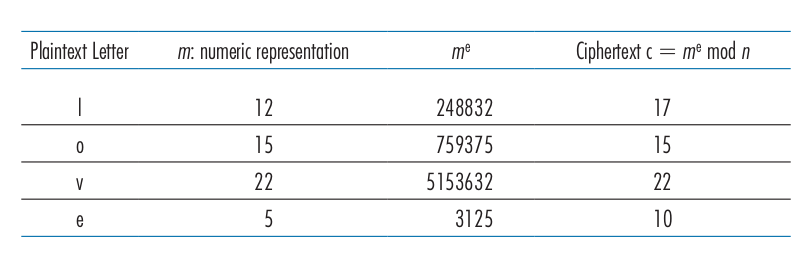
\includegraphics[scale=0.5]{Rsatab}\newline
\bf{Decryption Phase}\newline
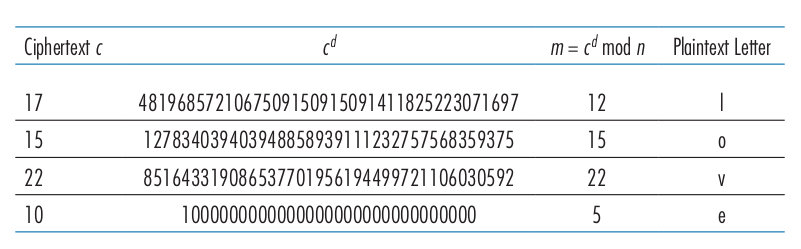
\includegraphics[scale=.5]{drcp}\newline
}\newpage
\subsection{How RSA Works!!}
\Large{In order to understand why RSA works, again denote n = pq,
where p and q are the large prime numbers used in the RSA algorithm.
Recall that, under RSA encryption, a message (uniquely represented by an integer),
m, is exponentiated to the power e using modulo-n arithmetic, that is,
$$c = m^e\;mod\;n$$
Decryption is performed by raising this value to the power d, again using modulo-n
arithmetic. The result of an encryption step followed by a decryption step is thus
$(m^e\;mod\;n)^d\;mod\;n$. Let’s now see what we can say about this quantity. As mentioned
earlier, one important property of modulo arithmetic is $(a\;mod\;n)^d\;mod\;n = a^d\;mod\;n$
for any values a, n, and d. Thus, using $a = m^e$ in this property, we have
$$\LARGE{\bf{(m^e\;mod\;n)^d \;mod \;n = m^{ed} \;mod \;n}}$$
It therefore remains to show that m ed mod n = m. Although we’re trying to
remove some of the magic about why RSA works, to establish this, we’ll need to use a
rather magical result from number theory here. Specifically, we’ll need the result that
says if p and q are prime, n = pq, and z = (p - 1)(q - 1), then $x^y$ mod n is the same as
$x^{(y \;mod \;z)}\; mod\; n$. Applying this result with x = m and y = ed we have
$$m^{ed}\; mod\; n = m^{(ed\; mod \;z)}\; mod\; n$$
But remember that we have chosen e and d such that ed mod z = 1. This gives us
$$m^{ed} \;mod\; n = m^1\; mod\; n = \;m$$
which is exactly the result we are looking for! By first exponentiating to the power of
e (that is, encrypting) and then exponentiating to the power of d (that is, decrypting),
we obtain the original value, m. Even more wonderful is the fact that if we first
exponentiate to the power of d and then exponentiate to the power of e—that is, we
reverse the order of encryption and decryption, performing the decryption operation
first and then applying the encryption operation—we also obtain the original value,
m. This wonderful result follows immediately from the modular arithmetic:
$$(m^d \;mod\; n)^e\; mod \;n = m^{de}\; mod \;n = m^{ed}\; mod\; n = (m^e\; mod\; n)^d \;mod \;n$$

}

\end{document}